% !TEX root = ../thesis.tex

\section{Implementation}
\label{sec:implementation}
This is the Implementation.

\subsection{Groundwork: CataRT Extension}
\label{subsec:implementation_catart}

- Max 7

\begin{figure}[!htb]
  \centering
  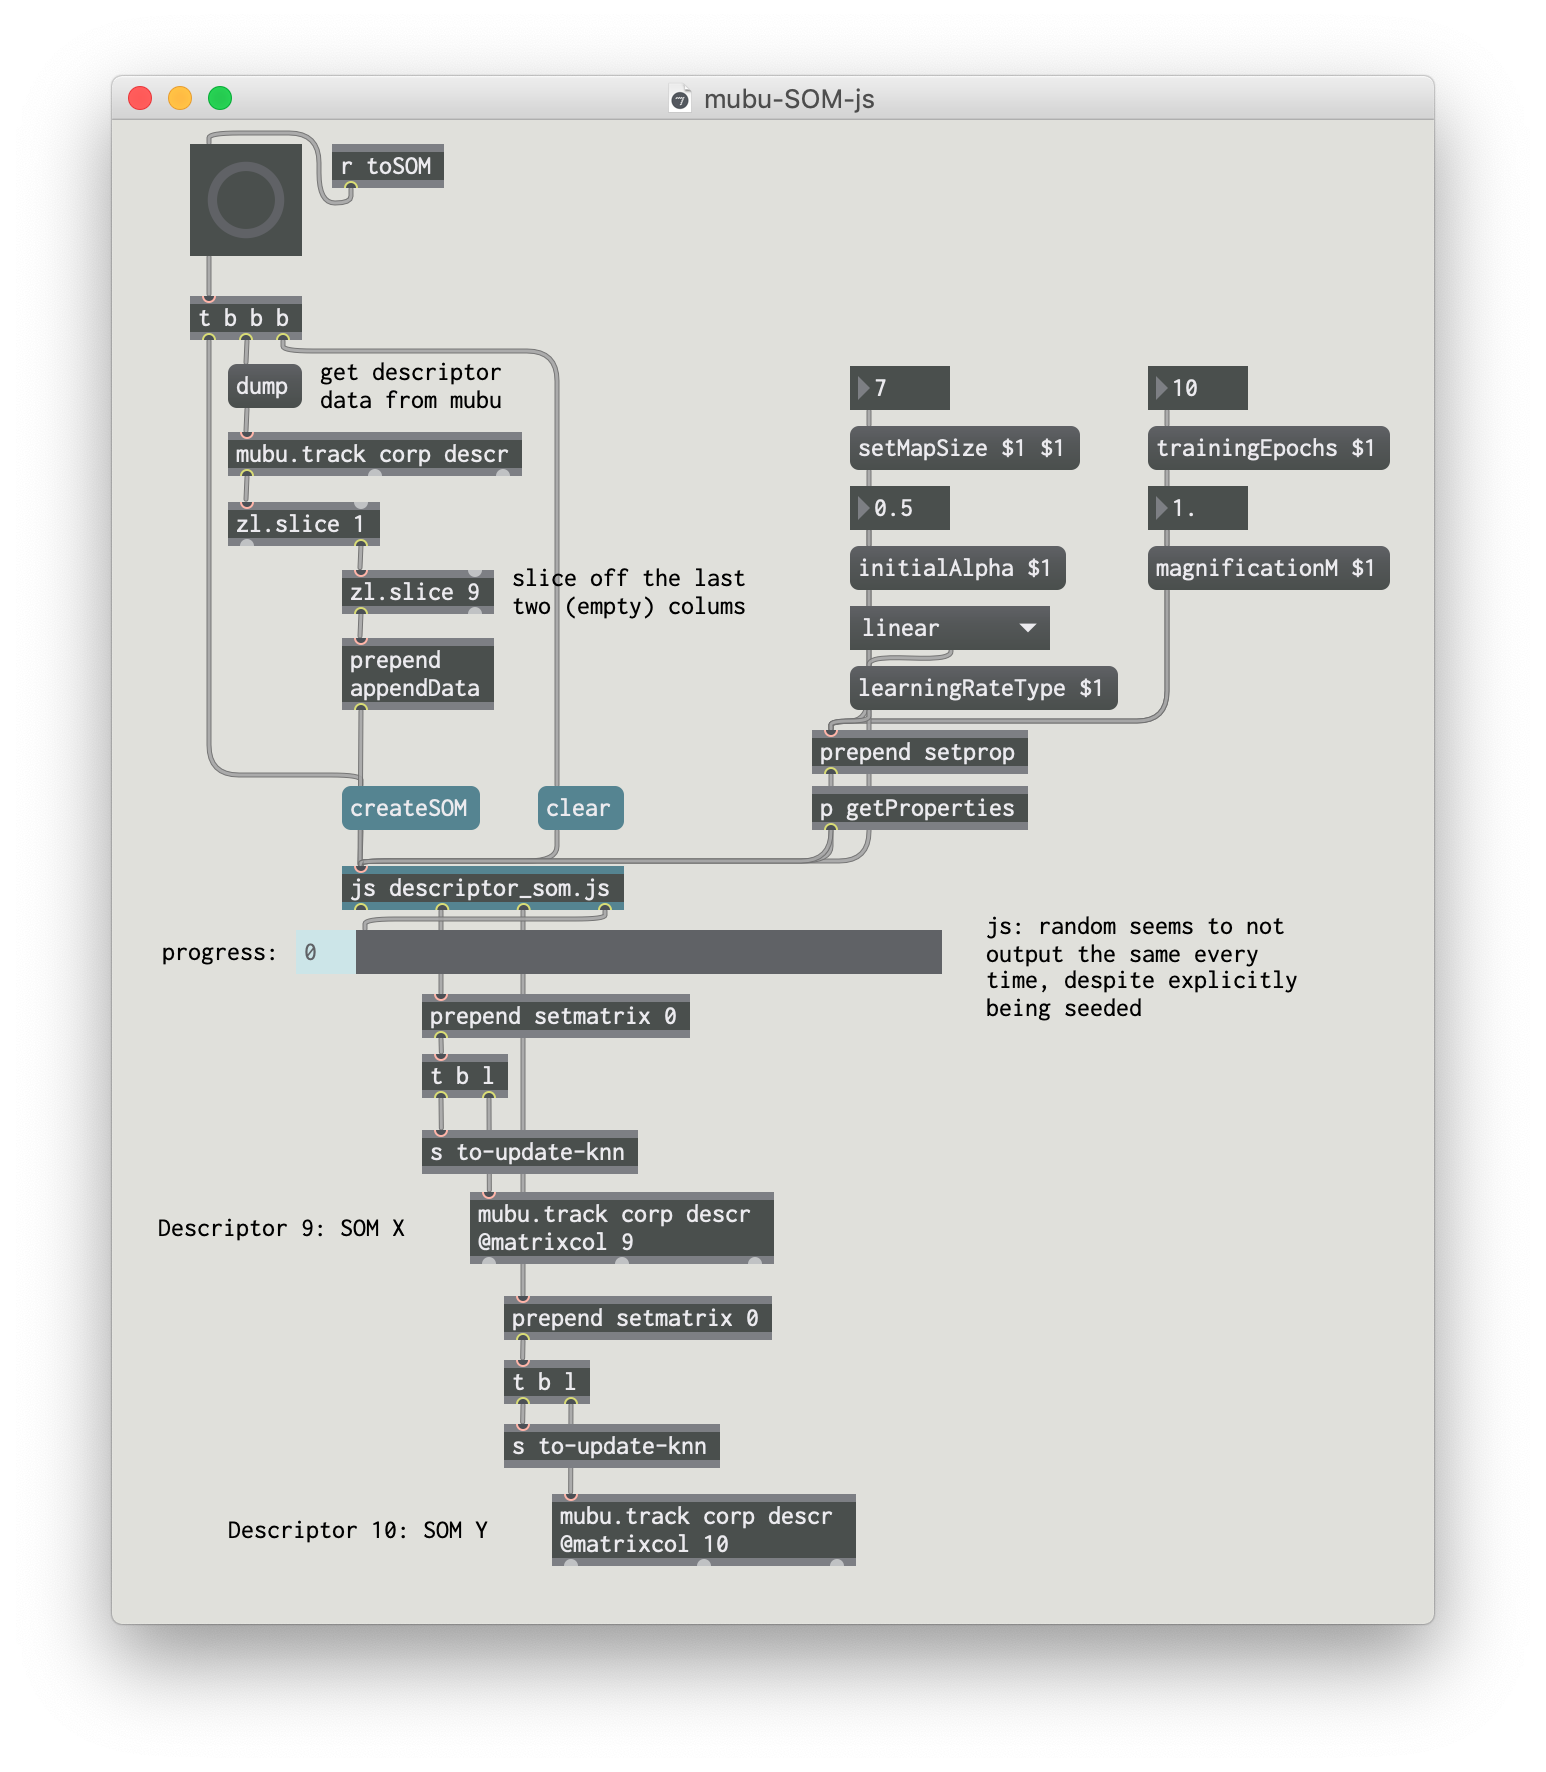
\includegraphics[width=\linewidth, trim=5mm 5mm 5mm 5mm, clip]{mubu-som-js}
  \caption{mubu-SOM-js}
  \label{fig:mubu-som}
\end{figure}

\subsubsection{Functionality}
\label{subsubec:mubu-som_functionality}

\subsubsection{Code Overview}
\label{subsubsec:mubu-som_overview}

main training loop:

\begin{listing}[!htb]
  \begin{mdframed}
    \inputminted[breaklines, numbers=left, firstline=306, lastline=312,
    fontsize=\footnotesize]{js}{../dev/mubu-som-js/descriptor_som.js}
  \end{mdframed}
  \caption{mubu-som-js/descriptor\_som.js: neuron position updates inside
  \mintinline{js}{trainingStep()}}
\end{listing}

\subsection{SOM Browser}
\label{subsec:implementation_som_browser}

\subsubsection{Functionality}
\label{subsubsec:som-browser_functionality}
desired functionality

\subsubsection{Libraries and Frameworks Used}
\label{subsubsec:som-browser_libraries}

\paragraph{Electron}
\label{para:electron}

\paragraph{React}
\label{para:react}

\paragraph{Web Audio API}
\label{para:web_audio_api}

\paragraph{Meyda}
\label{para:meyda}

choice of tools / frameworks:
- Electron
- React
- Web Audio (?)
- Meyda

what is application state?

\subsubsection{Application Structure}
\label{subsubsec:som-browser_structure}

Program structure:

\paragraph{System States}
\label{para:som-browser_states}
progression through system states

\paragraph{Background Processing}
\label{para:som-browser_background_processing}
background processing

\subsubsection{User Interface Components}
\label{subsubsec:som-browser_components}
App.js / components overview

\begin{listing}[!htb]
  \begin{mdframed}
    \inputminted[numbers=left, firstline=400, lastline=460,
    fontsize=\scriptsize]{jsx}{../dev/som-browser/src/components/App.js}
  \end{mdframed}
  \caption{som-browser/src/components/App.js:
  \mintinline{jsx}{<div className="AppContent">}}
  \label{lst:som-browser_app_content}
\end{listing}

\paragraph{TitleBar}
\label{para:title_bar}

\paragraph{MenuBar}
\label{para:menu_bar}

\paragraph{FileList}
\label{para:file_list}

\paragraph{Settings}
\label{para:settings}

\paragraph{Map}
\label{para:map}

\paragraph{FileInfo}
\label{para:file_info}

\paragraph{UserSelection}
\label{para:user_selection}
